\section{Introduction}
\label{sec:intro}

% ---
% Comments:
% What is the evidence that real distributed systems builders care about the properties we mention? Are there lots of papers on them or even references to docs of systems?
% What is the evidence that it's hard?
% ---
% Can we reduce jargon in the paper so people don't have to look up a zillion things?
% Can we provide references on the first mention of a term the reviewers might not know, such as causal consistency? Or if it's critical, even briefly explain it in words (e.g. consistency is about what values a client may see as it issues reads and write requests, e.g. does it ever see "stale" data after writing to an item).
% ---
% Why do we have to talk about confidential VM modules for example?
% Done
% ---
% \shubham{1. impl full then proof with no way to edit impl is not efficient and not sometimes doable also - waterfall - for the structure of the program proof can't be done, so we waste time implementing and proving it}
% \shubham{intuition for : }

% \shubham{2. much more clear and easier for non-formal people the advantage of this incremental}

% \shubham{3. what people understand: specs are procedures with pre and post. implementation is the filling these procedure and proof is what to prove?}

% \shubham{3a. lemma axiom, how are these matching to the use case? 
% }

% \shubham{4. proof synthesizer can work with partial implementations (holes). Proof synthesizer checks if this implementation matches the (pre/post) specification (what is this??).. decompose parts.}

% Axioms, lemmas

% \ion{While much better, one of my biggest concerns is that the paper is not yet written for the typical Neurips reviewer. It has too much jargon. For example, I am not sure how many AI outside of formal methods or programming languages communities actually know what "obligations", "axioms" or even "specifications" are.}


% Coding agents have made great strides at writing code for many tasks, as part of which they run tests and automatically refine their own output~\cite{cursor, claude-code, codex, swe-agent, reflexion}. They fall short, however, on tasks requiring correctness \textit{guarantees} across every possible behavior, not just the cases reached during testing. 
Coding agents have made great strides at writing code for many tasks, even running tests to automatically refine their own output~\cite{cursor, claude-code, codex, swe-agent, reflexion}. However, they fall short on tasks requiring correctness \textit{guarantees} across every possible behavior, rather than just the cases reached during testing.
Distributed systems are a prime example: properties such as consistency between subsequent writes and reads must hold under every possible interleaving of messages, failures, and concurrent updates, a combinatorially large space that no realistic test suite can cover~\cite{taxdc}. The consequences of incorrect behavior are severe, ranging from a replicated store that loses data~\cite{network_reliable}, to a file system that drops a write~\cite{all_not_equal}, to a confidential store that leaks a key.

% The consequences of incorrect behavior range 

% \shubham{people who have heard about formal methods, BUT NEVER used}
% \shubham{equivalent of waterfall? code generation and proof}
% \shubham{if something is non-provable (seemingly), then ur prove shows it does not work}
% \shubham{if u get a BIG BLOCK, its harder to locate the problem and to correct it}

% \shubham{compiler vs interpreter analogue?}
% \shubham{FIND ANALOGUES FOR ML PEOPLE}
% \shubham{sub-optimal than interleaved tasks}
% \shubham{Alex: AI driven discovery with which direction to move in might be useful here? 
% Ion: Its a iterative process.
% Alex: 
% Ion: Analogy: you want to capture the fact that its inefficient and its strictly worse!!
% Do one end to end, try to ask someone if its right and iterate.
% v/s
% you can check at each small step (each construct) not needing end to end.}

% \shubham{to be very clear about the cycle: how it helps the proof gen? 
% if I give the proof generation something that is extremely complex, finding proof might be just not doable.
% simpler, and ask to prove. I cna prove it I have this lemma.. and I can fill in for this lemma.. 
% you need to be very clear about how one HELPS another in SIMPLE terms. 
% }
% \shubham{specification: precoditiion post condition, obligation, properlty, ..}
% \shubham{what is a program, what are the constraints (for the input and output), what are the precoditions and post coditions.}
% \shubham{whois coming with the decomposition?}
% \shubham{Specs: what are the procedures, pre and post..and the implementation will be generated}
% \shubham{proof synth.. at a high level if every of this pre and post hold, I can prove it.. or we need decompose}
% \shubham{if a lemma is incorrect, it can just waterfall..}
% \shubham{partial implementations?
% can I prove end to end assuming that this is good..}

% Mechanized formal verification, or \textit{certification}, 
To prevent such catastrophic failures, formal verification techniques can provide exhaustive correctness guarantees. These techniques allow a developer to (1) state a specification, (2) write an implementation, and (3) develop a machine-checkable proof that the implementation satisfies the specification on every possible input~\cite{coq, lean, verus, dafny}.
%Landmark verified systems~\cite{sel4,compcert,fscq,ironfleet,verdi,chapar} have demonstrated feasibility, 
However, adoption of formal methods over the past two decades has been limited due to the immense manual labor required: verifying real-world systems takes months to years of expert effort~\cite{sel4,compcert,fscq,ironfleet,verdi,chapar}.
% However, adoption of formal methods over the past two decades has been limited because verifying real-world systems takes months to years of expert effort~\cite{sel4,compcert,fscq,ironfleet,verdi,chapar}.
% The verified distributed systems that do exist (e.g., IronFleet's Paxos~\cite{ironfleet}, Verdi's Raft~\cite{verdi}, Chapar's causal-consistency store~\cite{chapar}) have each demanded \emph{months to years} of human expert effort to write their proofs. 

% We show in \cref{sec:eval} that given access to a proof assistant and an iterative compile-and-feedback loop,

% give a coding agent a specification and formal verification tooling and ask it to build complex systems that provably satisfy the specification? 
Naturally, one may ask, can we simply provide a coding agent with a specification and formal verification tooling, and ask it to build complex systems that provably satisfy that specification? Our experiments demonstrate that the answer is no.
% We find the answer to be no. 
% In our tests (\cref{sec:eval}), 
We show in \cref{sec:eval} that Codex (GPT-5.4)~\cite{codex} and Claude Code (Opus 4.6)~\cite{claude-code} fail to generate correct systems for $5$ of $7$ widely studied distributed key-value-store consistency specifications (e.g., causal consistency, read-your-writes). The failure mode we observe is a structural one: following typical human patterns, agents treat verification as a downstream check on code they have already written. This approach (a) requires writing the whole proof at once, which is exceptionally difficult even for humans\footnote{Past work~\cite{chapar} reports 9--12 months of expert effort to write a proof for a key-value (KV) store.}, and (b) defers all correctness feedback to the end of an implementation, depriving the agent of valuable guiding signals. 
%As such, the agents often stalls on hard problems.


% This makes it easier to generate the proof, as each independet step is much less complex, and (b) guides implementation synthesis, as formal proof toosl can give partial feedback.

% Coding agents struggle to synthesize complex systems with formal proofs of correctness. 
% Note: Verification applied to synthesis was not reading well. We mean syntesize and verify.
% Even when given access to a proof assistant, SOTA coding agents Codex (GPT-5.4)~\cite{codex} and Claude Code (Opus 4.6)~\cite{claude-code}, succeed on only $2$ of $7$ widely studied distributed key-value-store consistency specifications (e.g., causal consistency, read-your-writes; \cref{sec:eval}). 

% \ion{We need a better way to state the limitations of this approach. Right now we say "implementation and proof are coupled, so we need to uncouple them", We need to say something like "This serial approach leads to needlessly spending resources to generate unprovable or very hard to prove code and makes it harder to correct the implementation in one shot. As such, the agents often stalls on hard problems.} 
% This serial approach leads to needlessly spending resources to generate unprovable or very hard to prove code and makes it harder to correct the implementation in one shot. As such, the agents often stalls on hard problems.
% But implementation and proof are tightly coupled; an agent that does not co-evolve them stalls on the obligations the spec imposes.

To address these challenges, we introduce \emph{Inductive Deductive Synthesis} (IDS), a technique that enables agents to synthesize provably correct complex systems from a specification. 
\begin{wrapfigure}{r}{0.525\linewidth}
\centering
\vspace{-0.8\baselineskip}
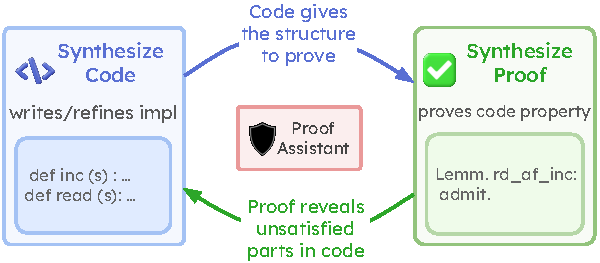
\includegraphics[width=\linewidth]{figures/img_intro.pdf}
\caption{\small Code and proof advance jointly and incrementally with IDS; the proof assistant grades each partial step. 
% \ion{I think that we need some names for the two boxes. It would make the explanation easier.}
% \mohsen{This figure is confusing. Do we need it?} \ion{I really think we need a figure. Please suggest a better one. Just draw it on a piece of paper and send out the picture.}
}
\label{fig:ids-intro}
\vspace{-0.8\baselineskip}
\end{wrapfigure}
% 
Our key insight is to synthesize both the implementation and its proof \textit{jointly and incrementally} (\cref{fig:ids-intro}), while learning from failures at each step to guide the search toward promising solutions and away from dead ends. As detailed in \cref{sec:background}, every implementation decision (e.g., adding a data structure or modifying control flow) is paired with a corresponding proof update (e.g., adding new constraints or splitting lemmas).
% As we show in \cref{sec:background}, in our approach, for each implementation decision (adding a data structure, modifying control flow, etc.), the agent correspondingly updates the proof (adding new constraints, splitting lemmas, etc.).

IDS offers two benefits: (1) each individual joint step is considerably simpler to \textit{prove}, decreasing the complexity of proof generation, and (2) the intermediate \textit{partial} proofs can be verified with a formal checker to assess the viability of the current design. A negative result rules out a dead-end implementation path before further work is wasted and serves as a counterexample to improve the design going forward.
% to report on the feasibility of getting to a correct implementation given the prior implementation decision; a \textit{no} rules out a dead-end search strategy before further work is wasted, and is provided to the agent as a counter-example to improve the strategy going forward. 
This is akin to ``chain-of-thought''~\cite{chain-of-thought},
except that the intermediate states are formally encoded and verified. %checkable for correctness. 
% \ion{The next sentence is confusing. What does extracted mean? compiled? If yes remove it, just say it is benchmarked. Also what does it mean for "proof to close"?} 
Beyond correctness, this iterative loop also optimizes performance: as soon as a candidate's implementation is complete, it is benchmarked on a distributed testbed; the performance measurements then further guide the search toward efficient implementations.
% Performance flows through the same loop: as soon as a candidate's implementation is complete, 
% it is benchmarked on a distributed testbed; the performance measurements then further steer the search towards efficient implementations.

% When deductive synthesis stalls, IDS employs an inductive feedback loop in the spirit of counter-example guided search~\cite{cegis,sketch,clarke2000counterexample}: an LLM agent analyzes previously failed strategies and pivots to more promising ones, such as proposing helper lemmas for stuck proofs.

% Our key idea is to synthesize the implementation and its machine-checkable proof \emph{jointly and incrementally} and to \emph{learn} using failures at each step as feedback to quickly steer the search toward promising strategies, away from dead ends.
%from failed attempts \ion{at each step} to \ion{quickly} steer the search toward promising strategies \ion{and thus avoid wasting computation in unpromissing directions}.
% 
% \green{An LLM agent incrementally develops a partial solution  that can have implementation placeholders with assumed specifications in the deductive-synthesis tradition~\cite{manna-waldinger,manna2006synthesis}). The proof that the partial implementation satisfies its specification can be tentatively constructed before the next steps prove that the placeholders satisfy their assumed specifications.
% 
% \ion{The rest of this paragraph doesn't say clearly why joint synthesis works. We need an explanation that can be understood by people who have never done formal spec/verification.}
% Unfilled work is staged as named placeholders (\texttt{Admitted} lemmas and stub bodies, in the deductive-synthesis tradition~\cite{manna-waldinger,manna2006synthesis}). 
% At every step the agent asks the type-checker whether the current partial implementation and proof can still extend to a complete pair; a \emph{no} rules out a dead-end design before further work is committed.}
% When deductive synthesis stalls, IDS employs an inductive feedback loop in the spirit of counter-example guided search~\cite{cegis,sketch,clarke2000counterexample}: an LLM agent analyzes previously failed strategies and pivots to more promising ones, such as proposing helper lemmas for stuck proofs.
% 
% Performance flows through the same loop: as soon as a candidate's implementation is complete, 
% it is extracted to executable code and benchmarked on a distributed testbed, even before its proof closes; the throughput then steers the search towards efficient implementations.
% so correctness and performance are co-optimized rather than sequenced.
% Note: correctness is optimized


% We apply LLM agents to synthesize the implementation and its proof \emph{jointly and incrementally}, in the deductive-synthesis tradition~\cite{manna-waldinger,manna2006synthesis}). 
% We use the proof assistant as a continuous oracle to check partial as well as complete candidates.
% Further we apply LLM agents to \emph{learn from failed proof strategies} and propose promising ones, in the inductive-synthesis tradition~\cite{cegis,sketch,clarke2000counterexample}. Incomplete lemmas and stub bodies are represented as named placeholders (\texttt{Admitted}), and at every step, the agent asks the type-checker whether the current partial pair can still extend to a complete proof; a \emph{yes} keeps a promising design alive, a \emph{no} drives exploration elsewhere.
% %  retrying with a new strategy.
% Performance flows through the same iterative process: 
% candidates are extracted to executable code, benchmarked on a distributed testbed, and their throughput is fed back as an additional signal towards efficient implementations.

% A pool of parallel \emph{Deductive Synthesis Agents} (DSAs) co-evolves implementation and proof under a \coq{} verification oracle. When a DSA stalls, an \emph{Inductive Synthesis Agent} (ISA) diagnoses the failure and responds: proposing helper lemmas for stuck proofs, or pivoting the design strategy for dead-end approaches.
%Before a candidate is accepted, a coordinator-side audit step verifies the proof is non-vacuous (e.g., that the specification was not modified and the implementation is non-trivial).

We instantiate \sys as a multi-agent system (\cref{sec:design}), and we evaluate \sys{} on 7 distributed key-value-store consistency specifications: Chapar's published causal-consistency spec~\cite{chapar} plus six new \emph{\sys{} suite} specs we release with the system (\cref{app:suite}). \sys{} produces a complete verified implementation on all 7 in about $6.8$ hours and \$$106$ per spec on average, with no human intervention or fine-tuning. On the two specs our vanilla agent baseline completed, \sys{} runs $1.6\times$ faster and $17\%$ cheaper. The discovered implementations match or beat hand-written expert references on every spec and reach up to $3\times$ the throughput of Chapar's published vector-clock reference, a margin we attribute to a design-space search broader than what manual proof allows.

As a general prover, \sys{} achieves state-of-the-art performance on four cross-language verification benchmarks (DafnyBench~\cite{dafnybench}, miniCodeProps~\cite{minicodeprops}, Verus-Bench~\cite{autoverus}, CoqStoq~\cite{rango}), beating agentic baselines that share its prompt and underlying model by $+10\%$ to $+51\%$. On three further code-and-proof synthesis benchmarks, \sys{} again leads: $176/189$ on VERINA~\cite{verina} (prior $38/189$), $65/77$ on AlgoVeri~\cite{algoveri} (prior $31/77$), and a perfect $62/62$ on CloverBench~\cite{clover}.

% \noindent In summary, we make the following contributions in this work:
% \begin{itemize}[leftmargin=*,nosep]
% \item \textbf{Inductive Deductive Synthesis (IDS):} a general technique combining incremental joint synthesis under a type-checker oracle (deductive) 
% with failure-driven improvement of the search strategy (inductive). 
% \ion{"implementation"? not sure what "strategy" means here} 
% \mohsen{search strategy for both the implementation and the proof.}
% \item \textbf{\sys{} system:} the first agentic LLM system to autonomously generate real-world distributed systems with end-to-end formal correctness guarantees.
% \item \textbf{\sys{} suite:} six \coq{} consistency specifications for distributed key-value stores, released for future verification/synthesis projects.
% \item 
% \ion{This is confusing. Maybe "\textbf{Couple performance with correctness:} use a real-world testbed to evaluate each correct implementation and steer the search toward efficient implementations."} 
% \mohsen{Agreed. This item seems odd. I think it is better to incorporate it with the first item IDS}
% \textbf{Performance in the loop:} throughput from a distributed-testbed steers the search to synthesize efficient implementations.
% % , so the loop co-optimizes correctness and performance.
% % Note: correctness is not optimized.
% \end{itemize}


\noindent In summary, we make the following contributions in this work:
\begin{itemize}[leftmargin=*,nosep]
\item \textbf{Inductive Deductive Synthesis (IDS):} the first general technique for jointly synthesizing code and machine-checked proof under a partial-proof oracle, with feedback from failures and performance benchmarks in the same loop.
\item \textbf{IDS-based multi-agent system:} the first agentic system to autonomously generate \textit{verified} distributed systems. Solves $7/7$ consistency specifications where SOTA agents (GPT-5.4, Opus 4.6) solve only $2/7$, with up to $3\times$ the throughput of published verified systems.
\item \textbf{\sys{} suite:} six new \coq{} specifications for distributed key-value-store consistency models, released as an open benchmark for verified-synthesis research.
\end{itemize}







